\chapter{Implementation}
\label{ch:implementation}

We implement our prototype in the LLVM framework, wasi-libc, and the wasmtime WebAssembly runtime.
The following sections detail the specific modifications and extensions we made to each component and some implementation choices and details to tackle specific problems.

\section{LLVM}
\label{sec:llvm}

We chose LLVM as our compiler, from C/C++ to WebAssembly.
We modify the existing \ac{WASM} backend and add support for the extension described in \cref{sec:wasm-extension}, allowing LLVM to emit the new instructions.

\subsection{LLVM IR}
\label{subsec:llvm-ir}

In the middle end, we introduce three new intrinsic functions that correspond and are lowered to our \ac{WASM} instructions by the backend.

\begin{itemize}
  \item[] \lstinline[style=customc,language=llvm]{ptr @llvm.wasm.segment.new(ptr, i64)}
  \item[] \lstinline[style=customc,language=llvm]{void @llvm.wasm.segment.set_tag(ptr, ptr, i64)}
  \item[] \lstinline[style=customc,language=llvm]{void @llvm.wasm.segment.free(ptr, i64)}
\end{itemize}

\noindent
The clang front end or a sanitizer pass can insert calls to these intrinsic functions.
\Cref{lst:llvm-intrinsics-float} shows how we lower a function that allocates 32 bytes on the stack to LLVM IR.

\begin{lstfloat}
  \begin{lstlisting}[frame=h,style=customc,
    label={lst:llvm-intrinsics},language=llvm]
  define hidden signext void @foo(i32 %index) {
  entry:
    %arr = alloca [32 x i8], align 16
    ; create a new segment
    %1 = call ptr @llvm.wasm.segment.new(ptr %arr, i64 32)

    ; do some work

    ; return ownership of segment to stack
    call void @llvm.wasm.segment.set.tag(ptr %1, ptr %arr, i64 32)
    ret void
  }
  \end{lstlisting}
  \caption{Code generated for a function that allocates 32 bytes on the stack.}
  \label{lst:llvm-intrinsics-float}
\end{lstfloat}

\subsection{LLVM Sanitizer Pass}
\label{subsec:llvm-sanitizer-pass}

\begin{table}[h]
  \centering
  \caption{Flags added to LLVM.}
  \label{tab:llvm-flags}
  \begin{tabular}{l | l | l}
    \textbf{Flag} & \textbf{Description} & \textbf{Required Flags} \\
    \hline
    \texttt{-mmem-safety}              & Enable the memory safety extension. & \\
    \texttt{-fsanitize=wasm-memsafety} & Enable the stack sanitizer. & \texttt{-mmem-safety} \\
  \end{tabular}
\end{table}

In LLVM, we introduce a \ac{WASM}-specific sanitizer pass that can be enabled via a compiler flag (see \cref{tab:llvm-flags}), designed to provide memory safety for stack allocations when compiling to WebAssembly.
This sanitizer analyzes functions for stack allocations, applies padding, and inserts calls to the intrinsics described in \cref{subsec:llvm-ir} to create segments, as discussed in \cref{subsec:stack-safety}.
The pass runs after all optimizations, ensuring we do not block passes that might remove stack allocations, such as \texttt{mem2reg}.

For each allocation the sanitizer hardens, we insert a call to the \texttt{segment.new} intrinsic after the allocation and replace all uses of the pointer to the allocation with our tagged pointer.
Before returns or tail calls, we need to return ownership of the segment to the stack frame, i.e.\ retagging using the stack pointers tag.
This serves two purposes: (1) subsequent code is able to access the memory through the stack pointer without a tagged pointer, and (2) use-after-return errors are caught, as the tagged pointer is not able to access the segment.

\subsection{C extension}
\label{subsec:c-extension}

To create and manipulate segments manually, e.g., to build a segment-aware memory allocator, we expose the memory safety features to C in the form of built-in functions that clang lowers to calls to the corresponding LLVM intrinsics.

\begin{itemize}
  \item[] \lstinline[style=customc]{void *__builtin_wasm_segment_new(void *, unsigned long);}
  \item[] \lstinline[style=customc]{void __builtin_wasm_segment_set_tag(void *, void *, unsigned long);}
  \item[] \lstinline[style=customc]{void __builtin_wasm_segment_free(void *, unsigned long);}
\end{itemize}

\noindent
The functions can be used as regular functions in C code, as illustrated in \cref{lst:builtin-functions-float}.

\begin{lstfloat}
  \begin{lstlisting}[frame=h,style=customc,
    label={lst:builtin-functions}]
  void *my_malloc(unsigned long size) {
    void *memory = malloc(size);
    return __builtin_wasm_segment_new(memory, size);
  }
  \end{lstlisting}
  \caption{Example of how a built-in function can be called from C.}
  \label{lst:builtin-functions-float}
\end{lstfloat}

\section{WASI Libc Modifications}
\label{sec:wasi-libc}

To allow us to run applications relying on libc on wasm64, we port the \acf{WASI} and wasi-libc to wasm64.
This work includes changing size and pointer types from 32 to 64\,bits.

We modify dlmalloc, the default allocator in wasi-libc, to provide memory safety for heap allocations.
We insert calls to the built-in functions exposed to C as necessary, creating memory segments and returning tagged pointers to these segments.
This protects both allocator metadata and adjacent allocations from being accessed or modified through heap overflows.
When freeing or reallocating memory, segments are freed, ensuring temporal safety.

\section{Wasmtime}
\label{sec:wasm-runtime}

\begin{table}[t]
  \centering
  \caption{Flags added to wasmtime.}
  \label{tab:wasmtime-flags}
  \begin{tabular}{l | l | l}
    \textbf{Flag} & \textbf{Description} & \textbf{Required Flags} \\
    \hline
    \texttt{-C mte}               & Enable the use of \ac{MTE}. & \\
    \texttt{-C mte-bounds-checks} & Use \ac{MTE} for bounds checks. & \texttt{-C mte} \\
    \texttt{-W mem-safety}        & Enable the memory safety extension. & \texttt{-C mte -W memory64} \\
  \end{tabular}
\end{table}

We implement our prototype in wasmtime\footnote{\url{https://wasmtime.dev/}}, a WebAssembly runtime with a focus speed and correctness, written in Rust.
Wasmtime features an optimizing compiler, cranelift\footnote{\url{https://cranelift.dev/}}, and its own \ac{IR}, \ac{CLIF}.

\begin{figure}[t]
  \centering
  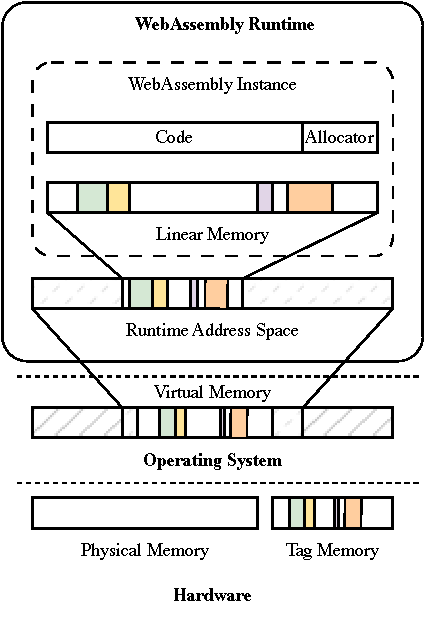
\includegraphics[scale=1]{figures/build/system-design-2}
  \caption{The memory safety extension, as implemented in wasmtime using \ac{MTE}. Memory segments are tagged, with different colors representing different tags. The processes virtual memory maps to physical memory and tag memory, which stores the tags assigned to memory granules.}
  \label{fig:wasmtime-mte-impl}
\end{figure}

In \cref{fig:wasmtime-mte-impl}, we can see an overview of our implementation of the memory safety extension in wasmtime using \ac{MTE}.
We modify wasmtime and its supporting libraries and extend it with support to parse and process the memory safety extension described in \cref{sec:wasm-extension}.
We add support for \ac{MTE} in the form of new instructions and lowering rules to cranelift, allowing wasmtime to generate \ac{MTE} instructions when compiling for a target that supports them.
We run in \ac{MTE} synchronous mode to catch and stop memory safety violations before their effects become observable to the violating or any other process.
These features can be enabled using the flags described in \cref{tab:wasmtime-flags}.

\begin{table}
  \centering
  \caption{Default tag $t$ for the linear memory.}
  \label{tab:default-tag}
  \begin{tabular}{c | c || c}
    \textbf{Memory Safety} & \textbf{MTE Sandboxing} & \textbf{Default Tag} \\
    \hline
    No  & No  & $t \in \{\,0\,\}$ \\
    No  & Yes & $t \in \{\,1, \dots, 15\,\}$ \\
    Yes & No  & $t \in \{\,0\,\}$ \\
    Yes & Yes & $t \in \{\,1\,\}$
  \end{tabular}
\end{table}

The memory is tagged by default with one of the tags described in \cref{tab:default-tag}, depending on the configuration.
This tag is then stored in the heap base pointer of the \ac{WASM} instance, allowing memory accesses through it.

For \ac{MTE}, we store the logical tag in the upper, unused bits of the \ac{WASM} index.
This index becomes a valid pointer once it is translated to an address by adding it to the heap base address.

In the following paragraphs, we will describe how we lower each of our instructions to an \ac{MTE} backend.

\paragraph{\texttt{segment.new}} To create a new segment, we (1) check that the requested segment is inside the linear memory for the guest, (2) generate a random logical tag and insert it into the index, and (3) set the allocation tag for the segment.
This involves generating a loop that iterates over the size of the segment and setting the tag using \texttt{stzg}, which also zeroes the memory.

\paragraph{\texttt{segment.set\_tag}} To change ownership of a segment, we again (1) check that the requested segment is inside the linear memory for the guest and (2) set the new allocation tag for the segment.
Here, we do not need to create a new, random tag, as we have passed a predefined tag.

\paragraph{\texttt{segment.free}} To invalidate a segment, we (1) check that the requested segment is inside the linear memory for the guest and (2) set the default allocation tag for the segment.
The default tag depends on the configuration and can be taken from \cref{tab:default-tag}.

\paragraph{}
We have implemented several optimizations to ensure our generated code runs efficiently.
When setting the allocation tag for a segment, we generate a loop iterating over the size of the segment.
If the size of the loop is known at compile time, we unroll the loop to tag up to 160\,bytes per iteration to avoid branch instructions.
We chose this tradeoff between code size and reducing the number of branch instructions executed.

When setting an allocation tag, we have four choices:
\begin{enumerate}
  \item \texttt{stg}: Setting the tag for a single tag granule,
  \item \texttt{st2g}: Setting the tag for two tag granules,
  \item \texttt{stzg}: Setting the tag for a single granule and zeroing the granule.
  \item \texttt{stgp}: Setting the tag for a single granule and storing a pair of registers.
\end{enumerate}

To ensure new segments are always zeroed, options 1) and 2) require an additional memset.
Our benchmarks for all four variants (see \cref{sec:mte-performance-evaluation}) show \texttt{stzg} as the variant with the lowest overhead while also clobbering one less register compared to \texttt{stgp}.

\subsection{Migration of the Linear Memory}
\label{subsec:migration-of-the-linear-memory}

When resizing linear memory, the runtime must relocate the existing contents and the \ac{MTE} tags if active.
We have two primary migration strategies (see \cref{fig:migrating-memory}).

\begin{figure}[h]
  \centering
  \begin{subfigure}[T]{0.45\textwidth}
    \centering
    \begin{lstlisting}[frame=h,style=customc,label={lst:migrating-memory-disable}]
disable_mte();
memcpy(from, to, len);
while from != end {
  asm!(
    "ldg {tag}, [{from}]",
    "stg {tag}, [{to}], #16",
    tag = out(reg),
    from = in(reg) from,
    to = inout(reg) to,
  );
  from = from.add(16);
}
enable_mte();
    \end{lstlisting}
    \caption{Code generated for the first migration approach.}
    \label{fig:migrating-memory-disable}
  \end{subfigure}
  \hfill
  \begin{subfigure}[T]{0.45\textwidth}
    \centering
    \begin{lstlisting}[frame=h,style=customc,label={lst:migrating-memory-tags}]
while from != end {
  asm!(
    "ldg {from}, [{from}]",
    "ldg {to}, [{from}]",
    "ldp {val1}, {val2}, [{from}]",
    "stgp {val1}, {val2}, [{to}], #16",
    from = in(reg) from,
    to = inout(reg) to,
    val1 = out(reg) _,
    val2 = out(reg) _,
  );
  from = from.add(16);
}
    \end{lstlisting}
    \caption{Code generated for the second migration approach.}
    \label{fig:migrating-memory-tags}
  \end{subfigure}
  \caption{Variants on how to migrate tagged memory.}
  \label{fig:migrating-memory}
\end{figure}

\begin{description}
  \item[Temporarily Disable \ac{MTE}:]
  Disable \ac{MTE} globally, copy memory and tags, then re-enable \ac{MTE}.
  This compromises memory safety during the migration for other threads in the same process relying on \ac{MTE} and can thus only be used if just a single \ac{WASM} instance is running.

  \item[Copy data and tags:]
  Load the memory tag for each 16\,byte granule.
  Use the tag to safely load and store data between memory regions, then set the tag for the new granule.

\end{description}

\noindent
We have measured the performance of both approaches in \cref{subsec:migrating-tagged-memory}.
As the approach to temporarily disable \ac{MTE} relies on just a single thread in the process requiring \ac{MTE} and is only marginally faster on some CPUs and slower on others, we choose the second approach.

\subsection{\ac{MTE} Sandboxing}
\label{subsec:bounds-checks}

In \cref{fig:system-design-sandboxing}, we show our approach to utilize memory tagging to replace software-based bounds checks.
The runtime assigns a tag (see \cref{tab:default-tag}) to each instance on module instantiation.
This tag is stored in the heap base address.
Memory access translation then involves adding the accessed index to the tagged heap base address.
The memory outside the linear memory, i.e.\ memory belonging to the runtime, is always tagged with the zero tag, ensuring \ac{MTE} catches accesses outside the sandbox and minimal modifications to the runtime.

However, we face a limitation in the number of sandboxes for this approach.
Since \ac{MTE} only offers up to 16 distinct tags, we are limited to up to 15 different sandboxes within one process, as we need to reserve one tag for the runtime.

\begin{figure}[t]
  \centering
  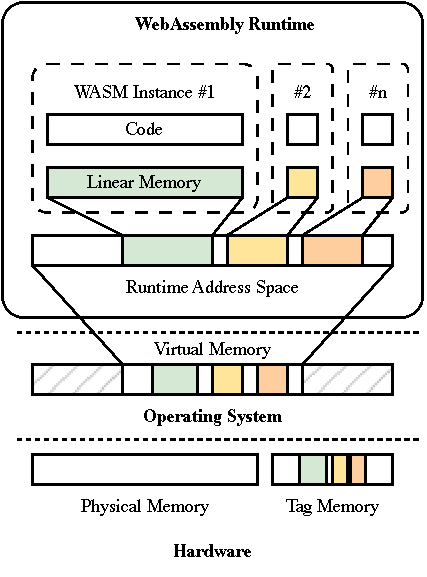
\includegraphics[scale=1]{figures/build/system-design-1}
  \caption{Bounds checks as implemented in wasmtime using \ac{MTE}. Each instances linear memory is assigned a unique tag, which re represent using different colors. The processes virtual memory maps to physical memory and tag memory, which stores the tags assigned to memory granules.}
  \label{fig:system-design-sandboxing}
\end{figure}

We can combine this approach with the memory safety extension by further restricting the number of sandboxes in one process and thus freeing up tag bits for the memory safety extension.
While it would be possible to assign up to three \ac{MTE} tag bits for sandboxing, we allocate three bits for the memory safety extension, thus just allowing a single instance to run in the same process.
We designate the lowest tag bit to determine whether memory belongs to the runtime or the linear memory.
Since we reserved the zero tag for the runtime, we tag the linear memory with the tag 1.
The remaining three tag bits used for the memory safety features can be generated by \texttt{segment.new}.
This results in memory indices always having an even logical tag, with the actual memory locations being assigned an odd allocation tag.

There are two challenges we need to take care of:
\begin{enumerate}
  \item Adding a tagged user pointer to the heap base address should be performant and result in the correct tag for the respective memory.
  \item Untrusted \ac{WASM} modules should not be able to forge tags that allow them to access memory beyond their allocated sandbox.
\end{enumerate}

As accesses are performed through integers, which code can arbitrarily change, adding an untrusted index to the heap base can be exploited to arbitrarily set the resulting logical tag, potentially allowing code to escape the sandbox.
To prevent this issue, we mask the tag bits allocated for the runtime from the index before address computation, as shown in \cref{fig:system-design-mem-safety-bounds}.
\Cref{fig:mte-bounds-checks} shows the masked bits when just \ac{MTE} bounds checking is enabled.
In this case, all tag bits are assigned for bounds checks and are masked out of the tag bits in the index.
In \cref{fig:mte-bounds-checks-mem-safety}, we see what happens when both \ac{MTE} bounds checking and memory safety are enabled.
Here, only the lowest bit is assigned for bounds checks, while the remaining three are assigned to the memory safety extension.
In \cref{tab:tag-mask}, we can see the mask used for each configuration.

\begin{table}
  \centering
  \caption{Tag mask for the index.}
  \label{tab:tag-mask}
  \begin{tabular}{c | c || c}
    \textbf{Memory Safety} & \textbf{MTE Sandboxing} & \textbf{Tag Mask} \\
    \hline
    No  & No  & -- \\
    No  & Yes & \texttt{and 0xF0FF\_FFFF\_FFFF\_FFFF} \\
    Yes & No  & -- \\
    Yes & Yes & \texttt{and 0xFEFF\_FFFF\_FFFF\_FFFF}
  \end{tabular}
\end{table}

\begin{figure}[t]
  \centering
  \begin{subfigure}[T]{\textwidth}
    \centering
    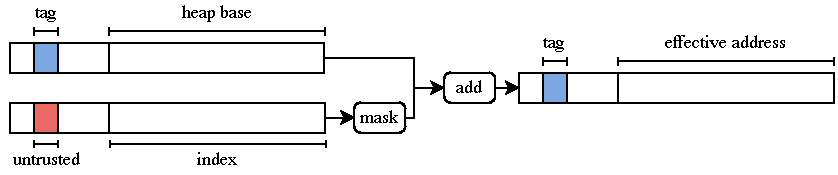
\includegraphics{figures/build/bounds}
    \caption{\ac{MTE} bounds checks.}
    \label{fig:mte-bounds-checks}
  \end{subfigure}
  \hfill
  \begin{subfigure}[T]{\textwidth}
    \centering
    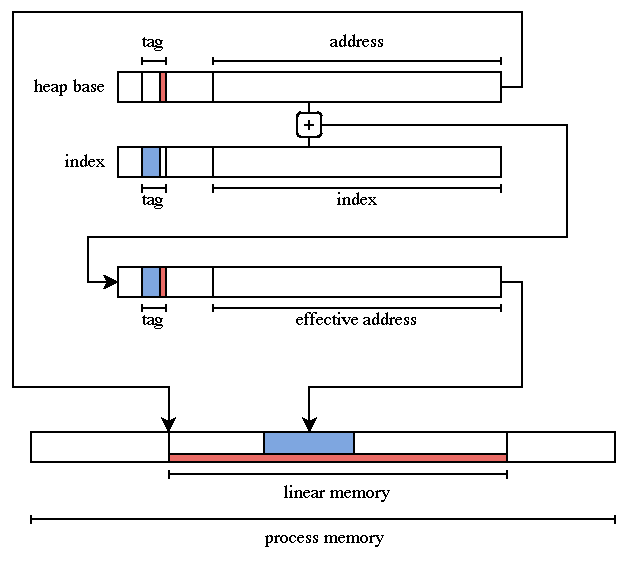
\includegraphics{figures/build/bounds-mem-safety}
    \caption{\ac{MTE} bounds checks with memory safety extension.}
    \label{fig:mte-bounds-checks-mem-safety}
  \end{subfigure}
  \caption{Effective address calculation with \ac{MTE} bounds checks.}
  \label{fig:system-design-mem-safety-bounds}
\end{figure}

\paragraph{Excluding Tags from Random Tag Generation}
If we are running with \ac{MTE} bounds checks enabled, we need a way to ensure to exclude certain tags from being generated by instructions such as \texttt{irg} (\textbf{i}nsert \textbf{r}andom ta\textbf{g}) or \texttt{addg} (\textbf{add} ta\textbf{g}).
These can be either specified as an exclude mask via an immediate to the instruction or an include mask via a \texttt{prctl} call, which sets a corresponding register in kernel space.
We choose the latter option and set the include mask at startup time.
In \cref{tab:tag-include-mask}, we list the include masks and included tags for the instructions mentioned above.
If the memory safety extension is disabled, none of these instructions will be emitted, so we do not need to exclude tags from being generated.

\begin{table}
  \centering
  \caption{Included tags for \texttt{irg}, \texttt{addg} instructions depending on configuration.}
  \label{tab:tag-include-mask}
  \begin{tabular}{c | c || c | c}
    \textbf{Memory Safety} & \textbf{MTE Sandboxing} & \textbf{Tag Include Mask} & \textbf{Included Tags} \\
    \hline
    No  & No  & -- & -- \\
    No  & Yes & -- & -- \\
    Yes & No  & \texttt{0xffff} & $t \in \{\,1, 2, \dots, 15\,\}$ \\
    Yes & Yes & \texttt{0x5555} & $t \in \{\,2, 4, \dots, 14\,\}$
  \end{tabular}
\end{table}

